\section{Simulation of the first controller}
Now we will simulate our system with the following initial conditions, and using the control law given in the previous part.
\begin{equation*}
    \begin{split}
        \phi(0) &= 10^{\circ} \\
        \theta(0) &= -5^{\circ} \\
        \psi(0) &= 15^{\circ} \\
        \boldsymbol{\omega}(0) &= \mathbf{0}
    \end{split}
\end{equation*}
To simulate this we first need to convert the initial conditions given in Euler angles to unit quaternions. We do this in the MATLAB script. See figure \ref{fig:eulang1} and \ref{fig:tau1} for the plots of the Euler angles and angular velocities ($\phi, \theta, \psi, \boldsymbol{\omega}$) and control inputs ($\boldsymbol{\tau}$).

We observe that the three angles $\phi$, $\theta$ and $\psi$, the three angular velocities $\omega_1$, $\omega_2$ and $\omega_3$ and the three control inputs $\tau_1$, $\tau_2$ and $\tau_3$ reach their desired values of 0 degrees, 0 degrees per second or 0 Nm. This happens after about 120 seconds. This is the behavior we expected because we have designed the closed-loop system to be stable.


\begin{figure}[h!]
    \centering
    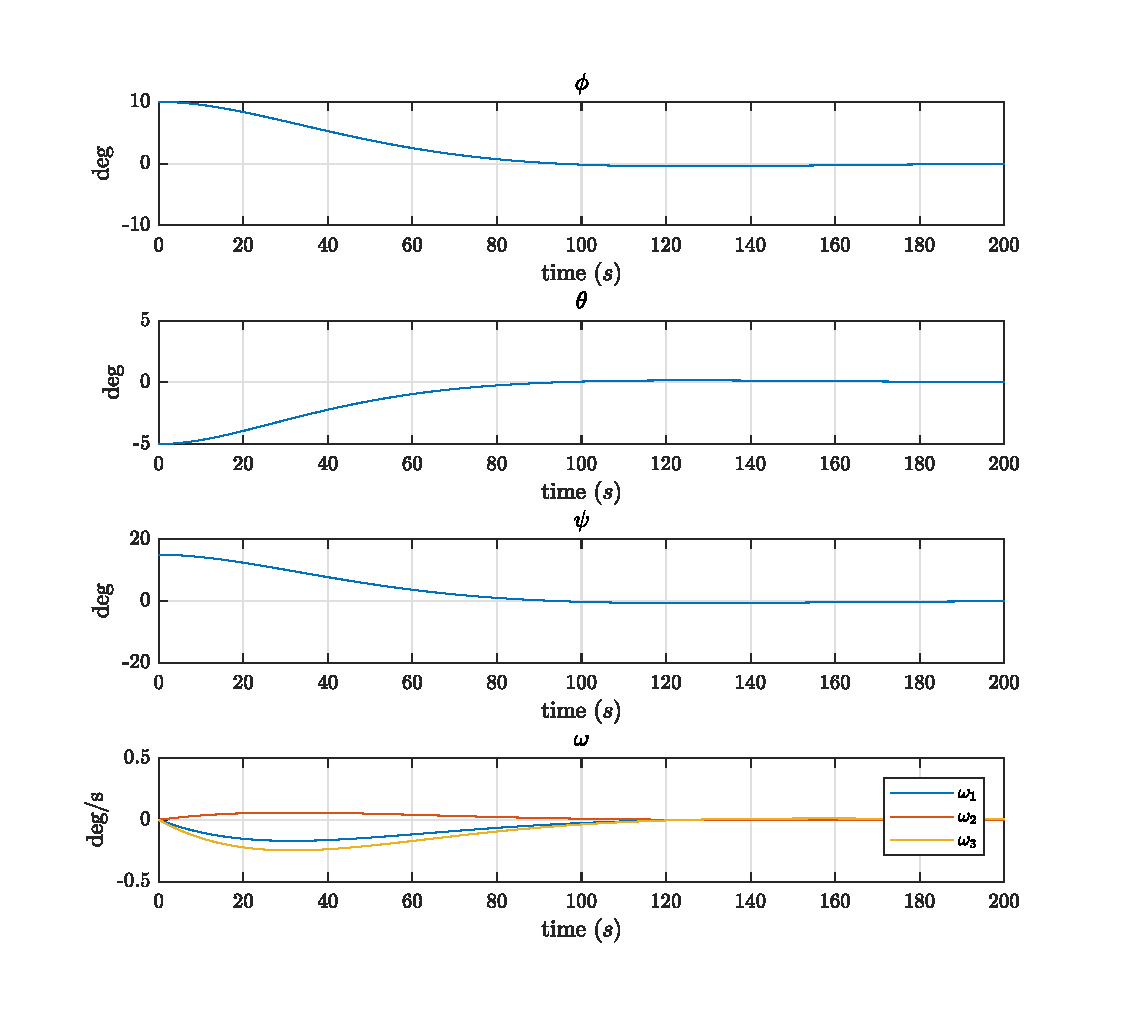
\includegraphics[scale=0.75]{eulang1.eps}
    \caption{Simluated Euler angles and angular velocity}
    \label{fig:eulang1}
\end{figure}


\begin{figure}[h!]
    \centering
    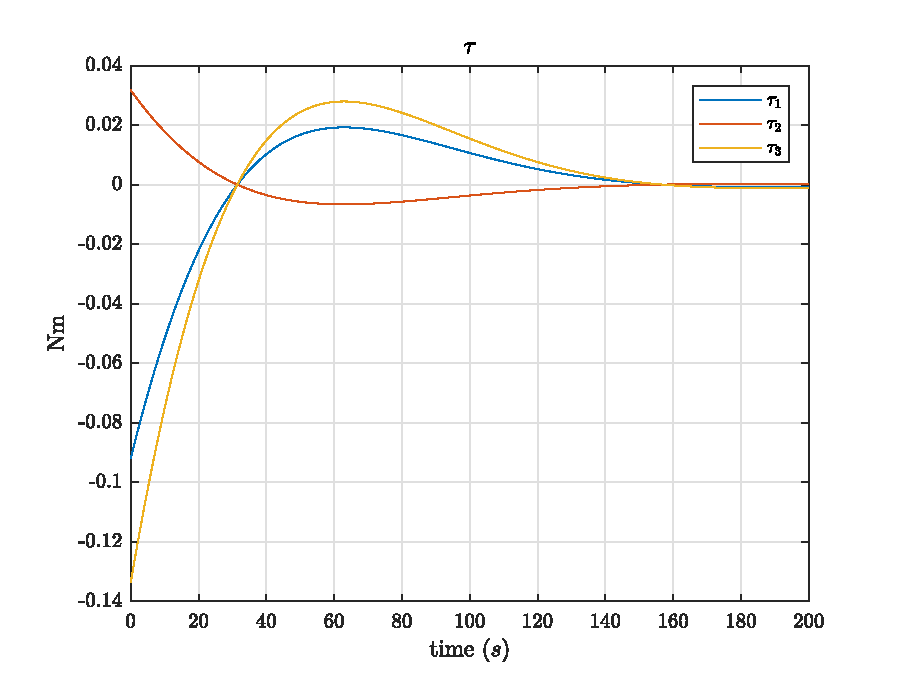
\includegraphics[scale=0.90]{tau1.eps}
    \caption{Simulated control input $\tau$ }
    \label{fig:tau1}
\end{figure}
